\chapter{Chapter}

\section{Introduction to the security of ICT systems}
Cybersecurity has become very important in today's world. Since every system relies on computer systems, any kind of damage can result in significant economic losses. Even indirect attacks that do not aim to steal money have economic costs. Cybersecurity is essential because attacks can be performed without the need to physically access the target location.


The reasons why cybersecurity is important are as follows:
\begin{itemize}
  \item Big damage on successful attacks
  \item Easy accessibility of systems
\end{itemize}

We must consider all the possible consequences of a successful attack. First, there can be \textbf{financial loss} (direct loss, for example, if someone gains access to bank account credentials, and indirect loss if the revelation that the company has been attacked negatively affects the stock exchange). There can be \textbf{recovery costs} because every successful attack results in damage, and there will be expenses required to return the system to normal operations and to enhance it to prevent new attacks. There can also be \textbf{productivity losses} if the attacks halt or delay processes. A successful attack may lead to \textbf{business disruption} because customers may seek alternative suppliers if a company is vulnerable to attacks.


For all these reasons we should protect systems. Most of the innovation is based on two main pillars:
\begin{itemize}
  \item The ability to communicate from any part of the world (communication networks)
  \item The increasing use of personal and mobile devices
\end{itemize}
These two foundations are no longer sufficient for innovative products; every new product now requires a security system.


\section{Complexity of the ICT scenario}
The ICT scenario is complex for various reasons. One key factor is the sheer number of different mobile and connected \textbf{devices}, including desktops, laptops, tablets, smartphones, smart TVs, fridges, and cars. All these devices can now connect to the internet, making security a critical concern.
\textbf{Communication networks } have shifted to data-only networks, meaning there are no more analog phone networks. This change implies that almost everything is vulnerable to potential attacks. It's not just wireless networks that can be targeted; even wired networks are susceptible to security threats.
\textbf{Distributed services} are on the rise, requiring constant technical solutions to keep them running. This often involves outsourcing parts of server management, hosting, and adopting cloud services. This means that computers are no longer confined within a company, which necessitates trust in the service providers. Additionally, software development is getting more complicated due to various factors like software layering, framework integration, and the use of multiple programming languages. This complexity increases the chances of errors and vulnerabilities.
In terms of security, the challenges can be summarized by the first engineering axiom:
\begin{center}
  "The more complex a system is, the harder it is to ensure its correctness."
\end{center}
Therefore, it's essential to keep systems as simple as possible. For instance, the number of bugs in a program tends to increase more than proportionally with the number of lines of code. The current complexity of information systems favors attackers, who can discover increasingly ingenious and unforeseen attack paths.\\
To express this idea clearly, we follow the \textbf{KISS rule}: \emph{"Keep it Simple, Stupid."}




% TMP old only
\ifthenelse{\boolean{showOld}}{
  \section{A definition of ICT Security}
  Each of us has a different concept of security: for example, the obligation to use safety belts when driving depends on country to country. Security is a personal concept but in engineering, we need to provide some formal definitions.
  Cybersecurity is a distributed part of a company, and every employee of a company must have the awareness for cybersecurity.
  \begin{enumerate}
    \item[1.] "Cybersecurity is the set of products, services, organization rules, and individual behaviors that protect the ICT system of a company."
  \end{enumerate}
  Let us explain the keywords in the definition.
  \begin{description}
    \item [Products:] refers to something that people can buy (such as products for firewall and VPN);
    \item [Services:] these services are implemented by buying products;
    \item [Organization rules:] they are required because even if, for example, a new system is set up with a password, rules must provide information to employees on how complex the password must be; otherwise, there will be no rules but personal behaviors, which could make the use of technical solutions less effective.
  \end{description}
  \begin{enumerate}
    \item [2.] It is the duty to protect the resources from undesired access, guarantee the privacy of information, ensure the service operation, and availability in case of unpredictable events (\textbf{C.I.A. = Confidentiality, Integrity, Availability}).
  \end{enumerate}

  More in detail, these three concepts have the following meaning:
  \begin{itemize}
    \item \textbf{Confidentiality} covers two related concepts:
          \begin{description}
            \item [Data confidentiality:] assures that private or confidential information is not made available or disclosed to unauthorized individuals.
            \item [Privacy:] assures that individuals control or influence what information related to them may be collected and stored and by whom and to whom that information may be disclosed.
          \end{description}
          In terms of requirements and the definition of a loss of security, it means preserving authorized restrictions on information access and disclosure, including means for protecting personal privacy and proprietary information. A loss of confidentiality is the unauthorized disclosure of information.

    \item \textbf{Integrity covers} two related concepts:
          \begin{description}
            \item [Data integrity:] assures that information (both stored and in transmitted packets) and programs are changed only in a specified and authorized manner.
            \item [System integrity:] assures that a system performs its intended function in an unimpaired manner, free from deliberate or inadvertent unauthorized manipulation of the system.
          \end{description}
          In terms of requirements and the definition of a loss of security, it means guarding against improper information modification or destruction, including ensuring information non-repudiation and authenticity. A loss of integrity is the unauthorized modification or destruction of information.

    \item \textbf{Availability:} assures that systems work promptly, and service is not denied to authorized users. In terms of requirements and the definition of a loss of security, it means ensuring timely and reliable access to and use of information. A loss of availability is the disruption of access to or use of information or an information system.
  \end{itemize}

  This definition is a good starting point for cybersecurity, but more than the C.I.A. triad is required; two of the most mentioned are as follows:

  \begin{itemize}
    \item \textbf{Authenticity:} the property of being genuine and being able to be verified and trusted; confidence in the validity of a transmission, a message, or message originator. This means verifying that users are who they say they are and that each input arriving at the system came from a trusted source.

    \item \textbf{Accountability:} the security goal that generates the requirement for actions of an entity to be traced uniquely to that entity. This supports non-repudiation, deterrence, fault isolation, intrusion detection and prevention, and after-action recovery and legal action.
  \end{itemize}

  \begin{enumerate}
    \item[1.] "The objective is to guard the information with the same professionalism and attention as for the jewels and deposit certificates stored in a bank caveau".
    \item[3.] "The ICT system is the safe of our most valuable information; ICT security is the equivalent of the locks, combinations, and keys required to protect it".
  \end{enumerate}

}{
  % else
}



\section{Risk estimation}

\begin{wrapfigure}{r}{0.55\textwidth}
  \centering
  \includegraphics[page=8, width = 0.55\textwidth]{\slides}
\end{wrapfigure}

Before setting up a defense, we must understand what the risks are. To make a risk estimation, it is good to start from the \textbf{service}. Once we know the service we need to protect, we must identify the assets used to provide that service, and there are four categories of assets: \textbf{ICT resources} (computers, disks, networks), \textbf{data} (not the disks but something intangible that could be deleted or modified), \textbf{location} (assets must be inside a protected room), and \textbf{human resources} (which means the group of people who possess the knowledge that must not be shared).

After considering the assets, the next step is to identify the events that could affect their normal operation. The first point is that each asset has some \textbf{vulnerabilities} (for example, disks that are vulnerable to physical damage like a hammer hitting the disk), and some vulnerabilities can pose a real \textbf{threat} depending on the environment. For example, if a disk is left in an open place, someone might use a hammer to damage the disk. However, if the disk is locked in a room where nobody can access it, the vulnerability still exists but is not a real threat.

\vspace{5mm}
So, the process of analyzing a service searching for risks take place as follows:
\begin{itemize}[]
  \item Find the \textbf{assets} of the service to be protected;
  \item Finding the \textbf{vulnerabilities} of each asset;
  \item Finding the \textbf{threats}, giving the way in witch the assets are used;
\end{itemize}

\vspace{5mm}
Once we identify the threats we must:
\begin{itemize}
  \item decide for each threat which \textbf{impact} it could have (what happens if disk is destroyed? If there's only one copy it could be a disaster, but if there are many that's not a problem)
  \item the \textbf{event probability} of the threat. This is the last point to get the \textbf{risk estimation}.
\end{itemize}

\bigskip
Recap of terminology:
\begin{description}
  \item[Asset:] the set of goods
  \item[Vulnerability:] weakness of an asset;
  \item[Threat:] deliberate action/accidental even that can procure the loss of a security property exploiting a vulnerability;
  \item[Attack:] threat occurrence (deliberate action);
  \item[(negative) Event:] threat occurrence
\end{description}


% TMP: new content
\ifthenelse{\boolean{showNew}}{
  \section{Risk management}
  To prioritize the risks, we can build a \textbf{risk assessment matrix} (or risk heat map):
  \begin{figure}[h]
    \includegraphics[page = 10,trim = 1cm 3cm 1cm 12cm, clip, width = \textwidth]{\slides}
  \end{figure}
} {}
% end TMP: new content


\section{Analysis and management of security}

\begin{wrapfigure}{l}{0.40\textwidth}
  \centering
  \includegraphics[page = 11,trim = 2cm 2.1cm 2cm 4cm, clip, width = 0.40\textwidth]{\slides}
\end{wrapfigure}
Risk estimation is only a piece for analysis and management of security. We can see that \textbf{assets}, \textbf{vulnerabilities}, \textbf{threats} give us the \textbf{risks} and then we start the \textbf{management} of the security. This means that for those risks that are not acceptable, either because they have high impact or high probability to end up in an attack, we need to select countermeasures and implement them. The last step is \textbf{audit}, that means that some independent person comes to check our work (if we correctly identified risks, selected the correct countermeasures, implemented them correctly).

In this course we will consider three of these blocks: vulnerabilities, the available countermeasures, and how to implement countermeasures.


\begin{wrapfigure}{o}{0.55\textwidth}
  \centering
  \includegraphics[page = 12,trim = 0.4cm 3.5cm 0.8cm 4cm, clip, width = 0.55\textwidth]{\slides}
\end{wrapfigure}
What is the correct step in the lifecycle of a system to implement security?\\
In brief, there is no single correct point for implementing security because it must be addressed at each stage of the design process.\\
In more detail, when we perform the \textbf{analysis of requirements} for our system, we must conduct a risk assessment; based on these risks, we can define security policies and procedures that we will apply throughout the rest of the system design.\\
When evaluating \textbf{technical options}, we also need to identify security products. For example, when choosing a database, we must consider security alongside other factors such as speed and cost. If we opt for a database that automatically encrypts data, we have already addressed a security concern. Conversely, if we choose a faster database that lacks an encryption system, we will need to design that separately, incurring additional costs and efforts. \\
When \textbf{designing} the services that the system will offer, we must also include the security services component. Security should be integrated at each stage of the design process, not added as an afterthought. If we create a prototype website or app without any security measures, it will be challenging to retrofit security later on.


\section{Relation in the security field}
During the development of our system, we must integrate security at each step and ensure that the design is correctly implemented. We must test the system, including its security aspects. An example of this is testing against unexpected inputs to ensure that the system does not accept and process incorrect inputs.

While implementing our system, it is important to establish security mechanisms. Some systems include security functions, but they are often deactivated due to associated costs (generally, activating security may slow down the system). For instance, the default password of a home router may be shared among different units, so it is necessary to change that password.

When the system is operational, security must be managed on a daily basis, as the security landscape changes constantly.


\section{Relation in the security field}

The black box is the system itself.
Assets are exposed to vulnerabilities, and those vulnerabilities increase security risks.
Additionally, threats exploit vulnerabilities, and the existence of vulnerabilities creates the opportunity for a threat.
\begin{wrapfigure}{l}{0.55\textwidth}
  \centering
  \includegraphics[page = 14,trim = 1cm 3cm 1cm 5cm, clip, width = 0.55\textwidth]{\slides}
\end{wrapfigure}
On the left, there are the security requirements that we want to implement. Security requirements are indicated by security risks, and security requirements are met by security controls.

The \textbf{security control} is the most important piece of the picture nowadays. It is an element placed in the system to protect against a specific threat and reduce the risks to which the system is exposed. Examples of security controls include firewalls, VPNs, and disk encryption.

\bigskip
Some terminology:
\begin{description}
  \item[Incident:] A security event that compromises the integrity, confidentiality, or availability of an information asset (generic definition).
  \item[(Data) breach:] An incident that results in the disclosure or potential exposure of data.
    \begin{itemize}
      \item Disclosure: Occurs when data is intentionally given to someone.
      \item Exposure: Data becomes available to anyone who knows where to find it.
    \end{itemize}
  \item[(Data) disclosure:] A breach for which it is confirmed that data was actually disclosed (not just exposed) to an unauthorized party.
\end{description}
The difference between the last two is that the last one is a breach involving data that were not just exposed but also confirmed to be disclosed to an unauthorized party.


\newpage
\section{Window of exposure}
\begin{wrapfigure}{r}{0.60\textwidth}
  \centering
  \includegraphics[page = 16,trim = 0.2cm 1.7cm 0.2cm 4cm, clip, width = 0.60\textwidth]{\slides}
\end{wrapfigure}
The \textbf{window of exposure} is \emph{the time between the discovery of a new vulnerability and the installation of a patch}.


Analyzing the graph from the left, we notice a consistently low level of risk, which, although it can never be reduced to 0, remains close to it.
However, at a certain juncture, a new vulnerability is discovered, causing the risk to surge due to its uncontrollable nature.
At a specific point (marked as the red point), an individual exploits this vulnerability to execute an attack. This action leads to the vulnerability becoming public, thereby making it accessible to everyone.
This initial stage is commonly referred to as \textbf{discovery}.

After an attack is carried out, two distinct groups of individuals become aware of it: the \emph{bad guys} who aim to compromise the system and the \emph{good guys} who strive to safeguard the system. Within these two categories, there is also the product vendor, who must be informed of the vulnerability. The vendor should, in turn, promptly notify its customers of the newly discovered vulnerability. While the vendor is working on fixing the vulnerability, users of that product should refrain from attempting to fix it, which is typically impossible. Instead, they should focus on updating their security tools, at the very least, to detect if the vulnerability is actively being exploited in attacks. This is the \textbf{publication} phase during which the vulnerability becomes public knowledge, and everyone is awaiting a fix while also making efforts to detect potential attacks.

Finally, at some point in time, the vendor creates a patch to fix the vulnerability. However, the patch must be distributed, and the risk only decreases when the patch becomes widely known and is eventually installed, rendering the system \textbf{protected}. The window of exposure can persist for days or even months, which is why security is an ongoing effort.

\section{Some statistics}
\begin{wrapfigure}{r}{0.55\textwidth}
  \centering
  \includegraphics[page = 17,trim = 1cm 2.6cm 1cm 7cm, clip, width = 0.55\textwidth]{\slides}
\end{wrapfigure}
The graphic shows that there are about 10 million attacks per month using malware. That is why we should always keep our anti-virus/anti-malware updated.
If we consider web servers across all sectors, 44\% of servers were consistently vulnerable to attacks every day of the year.
\begin{figure}[h]
  \centering
  \includegraphics[page = 18,trim = 1cm 1.7cm 1cm 7cm, clip, width = 0.60\textwidth]{\slides}
\end{figure}

The term \textbf{0 day} refers to the first day when a vulnerability is reported to the public and has not yet been fixed.

The banking sector boasts the best security track record, with the lowest vulnerability rate (rarely vulnerable for 30 days or less each year).

In general, achieving strong security is challenging. Vulnerabilities can be discovered by both well-intentioned individuals (good guys) and malicious actors (bad guys). Some people investigate software to uncover vulnerabilities and inform the vendor to patch them before they are exploited by malicious actors. This proactive approach is taken to ensure patches are in place before vulnerabilities are discovered by the bad guys.

The "\textbf{0-day initiative}" (\textbf{ZDI}) discovers vulnerabilities and notifies the relevant organizations \emph{before} making them public. ZDI typically provides a 120-day grace period from the discovery of a new vulnerability to allow the vendor to fix it before disclosing it to the public. Longer deadlines can be risky, as bad guys may discover the vulnerability during the extended time frame.

\vspace{5mm}
Example:
\begin{itemize}
  \item 8 May 18: ZDI reports the vulnerability to the vendor, and the vendor acknowledges the report.
  \item 14 May 18: The vendor replies that they have successfully reproduced the issue reported by ZDI.
  \item 9 Sep 18: The vendor reports an issue with the fix and states that the fix might not be included in the September release.
  \item 10 Sep 18: ZDI issues a caution about a potential 0-day (which means that the vulnerability, for which a fix is not available, is going to be published).
  \item 11 Sep 18: The vendor confirms that the fix did not make it into the build.
  \item 12 Sep 18: ZDI confirms its intention to 0-day on 20 Sep 18.
\end{itemize}

% TMP: new part
\ifthenelse{\boolean{showNew}}{
  \section{Cyber threats}

  \subsection*{Components}
  \begin{wrapfigure}{r}{0.30\textwidth}
    \centering
    \includegraphics[page = 20,trim = 8cm 3cm 8cm 11cm, clip, width = 0.30\textwidth]{\slides}
  \end{wrapfigure}
  There are \textbf{three main components} in cyber threats:
  \begin{itemize}
    \item threats actors (and their motivation)
    \item attack vectors (vulnerabilities and context)
    \item vulnerable targets (value for owner and attacker)
  \end{itemize}


  \subsection*{Motivations: \emph{MICE}}
  What are the motivations behind this?
  \begin{itemize}
    \item \textbf{M is for Money:} direct transfer, blackmail, ... or indirect (e.g. data reselling);
    \item \textbf{Is is for Ideology:} political, religious, hacktivism;
    \item \textbf{C is for Compromise:} individuals with no choice due to blackmail or threat against their families or themselves;
    \item \textbf{E is for Ego:} bragging around and positive reputation, "we do it because we can".
  \end{itemize}
  \begin{figure}[h]
    \includegraphics[page = 21,trim = 22cm 2.1cm 1cm 12cm, clip, width = 0.10\textwidth]{\slides}
  \end{figure}
  \begin{figure}[h]
    \centering
    \includegraphics[page = 22,trim = 1cm 2.1cm 1cm 4cm, clip, width = 0.50\textwidth]{\slides}
    \caption{Threat actors}
  \end{figure}


  \subsection*{Standardization bodies}
  Standardization bodies in cybersecurity are organizations that develop and publish standards and guidelines to enhance security and interoperability in computer systems and networks.
  %TODO: might be better to add subfigures here
  \begin{figure}[!h]
    \centering
    \includegraphics[page = 23,trim = 1cm 3cm 1cm 2cm, clip, width = 0.50\textwidth]{\slides}
    \includegraphics[page = 24,trim = 1cm 3cm 1cm 2cm, clip, width = 0.50\textwidth]{\slides}
  \end{figure}
} {}




\section{What is Security?}
\begin{quote}
  "Security is a process, not a product".
  \begin{flushright}
    (Bruce Schneier, Crypto-Gram, May 2005)
  \end{flushright}
\end{quote}


If we have learned anything from the past couple of years, it is that \textbf{computer security flaws are inevitable}.
Systems break, vulnerabilities are reported in the press, and still many people put their faith in the next product, or the next upgrade, or the next patch. "This time it's secure," they say. So far, it has not been.
\textbf{Security is a process, not a product}. Products provide some protection, but the only way to effectively do business in an insecure world is to put processes in place that recognize the inherent insecurity in the products.
\textbf{The trick is to reduce your risk of exposure regardless of the products or patches}.

\subsection*{Security Principles}
To make it possible, it is necessary to follow some security principles:
\begin{itemize}
  \item \textbf{Security in depth}: if the enemy can defeat the first line of defense, there must be a second line to stop the attacker. Do not rely on just one defense, as that defense may have a bug or problem. It is better to have multiple levels of defense, so as the attacker breaks through the defenses, it will become increasingly difficult to keep penetrating.

  \item \textbf{Security by design}: this means that the security design is integrated into the system from the beginning and not added as an afterthought.

  \item \textbf{Security by default}: users should not have the choice to activate or deactivate security. Security should be enabled by default, and it should require significant effort to disable security features.

  \item \textbf{Least privilege}: this principle dictates that any element operating within the system should be assigned the minimum amount of privileges necessary to perform its task. Imagine a scenario where a system has excessive privileges, and it is being attacked by a virus. The virus could gain access to everything because of the excessive privileges.

  \item \textbf{Need-to-know}: this principle emphasizes that access to any component of the system should be granted only for the data required to execute a specific task. For example, in the case of Amazon, several people work within the system. When a customer places an order on Amazon, the first person handling the order can only see the details of what was ordered. They do not have access to information about who placed the order or the destination of the goods.
\end{itemize}

% TMP: old content1
\ifthenelse{\boolean{showOld}}{
  \subsection*{European Central Bank}
  ECB made on 31/01/2013 some "\emph{Recommendations for the security of Internet payments}". In general, when there is a regulation there are \textbf{generic} recommendations, but typically lawyers do not want to get into details. In the security scenario this is changed recently. It is not possible to let individual companies decide what are the good rules for security. These recommendations apply to payment schemas governance authorities, payment service providers (PSP), and merchants that use credit cards for payments.

  The main recommendations are:
  \begin{itemize}
    \item Protect the initiation of Internet payments, as well as access to sensitive payment data, by \textbf{strong customer authentication};
    \item \textbf{Limit the number of log-in or authentication attempts}, define rules for Internet payment services session “time out,” and set time limits for the validity of authentication;
    \item Establish \textbf{transaction monitoring mechanisms} designed to prevent, detect, and block fraudulent payment transactions (reminiscent of Security in depth);
    \item \textbf{Provide assistance} and guidance to customers about best online security practices, set up alerts, and provide tools to help customers monitor transactions.
  \end{itemize}
}{}

\section{Security properties}
\begin{center}
  \begin{tabular}{||l l||}
    \hline
    Authentication (simple/mutual)             & autenticazione (semplice/mutua)         \\
    Peer authentication                        & autenticazione (della controparte)      \\
    Data/origin authentication                 & autenticazione (dei dati)               \\
    Authorization, access control              & autorizzazione, controllo accessi       \\
    \textbf{Integrity}                         & \textbf{integrità}                      \\
    \textbf{Confidentiality, privacy, secrecy} & \textbf{riservatezza, confindenzialità} \\
    Non-repudiation                            & non ripudio                             \\
    \textbf{Availability}                      & \textbf{disponibilità}                  \\
    Traceability, accountability               & tracciabilità                           \\
    \hline
  \end{tabular}
\end{center}


\subsection{Peer authentication}

\subsubsection*{Simple peer authentication}

% Using minipage 
\noindent
\begin{minipage}{0.5\textwidth}
  \centering
  \includegraphics[page = 29,trim = 1cm 3cm 1cm 5cm, clip, width = \linewidth]{\slides}
\end{minipage}
\hspace{0.05\textwidth}
\begin{minipage}{0.4\textwidth}
  When there is communication between two peers that take part in the communication, they must authenticate. Two entities are considered peers if they implement the same protocol on different systems; for example, two TCP modules in two communicating systems. Computer systems usually ask some questions like the ones in the picture. Typically, for a proof, we provide a password. This is simple authentication: only one party authenticates. It attempts to provide confidence that an entity is not engaging in either masquerade or an unauthorized replay of a previous connection.
\end{minipage}


\subsubsection*{Mutual peer authentication}
\noindent
\begin{minipage}{0.5\textwidth}
  \centering
  \includegraphics[page = 30,trim = 1cm 3cm 1cm 4.5cm, clip, width = \linewidth]{\slides}
\end{minipage}
\hspace{0.05\textwidth}
\begin{minipage}{0.4\textwidth}
  In mutual peer authentication, we also require a formal proof that we are connected to the real server. A fake server could display the same page as the ordinary bank just to obtain credentials from the user. When we connect to a server, we typically trust the server, but we need proof. Both parties authenticate each other.
\end{minipage}

\subsubsection*{Data origin authentication}
\noindent
\begin{minipage}{0.5\textwidth}
  \centering
  \includegraphics[page = 31,trim = 1cm 3cm 1cm 4.5cm, clip, width = \linewidth]{\slides}
\end{minipage}
\hspace{0.05\textwidth}
\begin{minipage}{0.4\textwidth}
  Someone could write an email to request an increase in someone's salary, signed by the director, but there is no proof that the email came from the director. An electronic email typically lacks proper authentication. The same issue applies to files. Data are usually not authenticated, so there is a need for an authentication system for data as well.
\end{minipage}

\subsection{Non-repudiation}
Non-repudiation is a \textbf{formal proof} that is admissible in a court of law, providing \textbf{undeniable evidence of the data's creator}. Non-repudiation prevents either the sender or receiver from denying a transmitted message. This has several implications because we not only need \textbf{authentication} but also \textbf{integrity}. If someone alters data in a document, it should be detectable because it is no longer the original authenticated document.

There is a difference between authentication and identification. Authentication involves using electronic means to verify identity, such as a username and password. However, if the password is stolen, it raises doubts about whether it is the legitimate user or someone else. On the other hand, identification is much stronger, as seen in technologies like the Touch ID on smartphones, where the user is the only one capable of performing that operation.

\textbf{Beware!} The concept of "non-repudiation" is typically associated with not only technical aspects but also with specific procedures carried out voluntarily. We rarely achieve non-repudiation with protocols or procedures that automatically perform actions on behalf of the user.

\subsubsection*{Example of non-repudiation}
%&& !inSnippetMode
Let's consider non-repudiation of an electronic signature:
\begin{itemize}
  \item Syntax (is that your signature?)
  \item Semantics (did you understand what you were signing?) - what you don't understand has no legal value (for example the small lines in a document that are not understandable).
  \item Will (have you signed voluntarily?)
  \item Identification (was really YOU the signer?)
  \item Time (when did you sign?)
  \item Place (where did you sign?)
\end{itemize}
The electronic signature is a set of bits that represent the signature of a person. If we do not know where these bits must be placed to represent the signature, we cannot know which person the signature belongs to. For these reasons, there are specifications for electronic signatures.


\subsection{Availability}
An availability service is one that protects a system to ensure its availability. This service addresses the security
concerns raised by denial-of-service attacks. It depends on proper management and control of system resources
and thus depends on access control service and other security services.


\subsection{Authorization (access control)}
\begin{wrapfigure}{r}{0.55\textwidth}
  \centering
  \includegraphics[page = 33,trim = 0.3cm 2.7cm 3cm 4.5cm, clip, width = 0.55\textwidth]{\slides}
\end{wrapfigure}
Authentication means identifying the actors in the system. After authentication, we can make decisions. For example, in the figure, Barbara has correctly identified herself and then asks the computer to "open the box of Alice's car" and the computer performs an \textbf{authorization decision (or access control)}. This is because the car in the box does not belong to Barbara. Therefore, a system must also determine if someone is authorized to perform an operation or not.

\subsubsection*{Important difference!}
\begin{itemize}
  \item \textbf{Authorization} is the process of verifying whether you, who have already been authenticated, are permitted to perform a particular operation.
  \item \textbf{Authentication} is the process of identifying the users of a system.
\end{itemize}

\ifthenelse{\boolean{showOld}}{
  \subsubsection*{Pyramid of security}
  \begin{figure}[h]
    \centering
    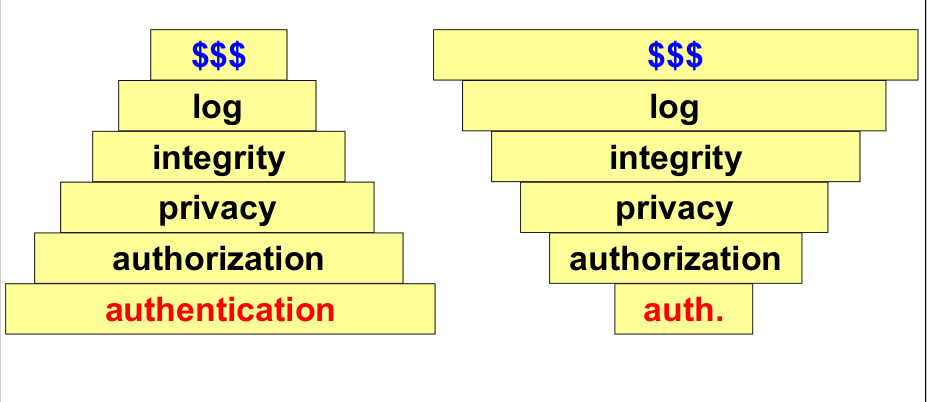
\includegraphics[trim = 0.2cm 0cm 0.2cm 0cm, clip, width = 0.55\textwidth]{chapter1/pyramid_of_security.png}
  \end{figure}
  Authentication is the most fundamental feature in our system. Without the ability to identify the actors, we cannot establish a strong security foundation. Building upon authentication, we have:
  \begin{itemize}
    \item Authorization (who can perform specific actions),
    \item Privacy (who can access data),
    \item Integrity (who can modify data), and
    \item Logging (keeping records of actions).
  \end{itemize}
  Unfortunately, many systems rely on weak authentication methods, often limited to just usernames and passwords. This weak link can undermine the entire security structure. This is a common issue in many organizations, as managers may not fully grasp the technical principles necessary to understand how these various security mechanisms work together.
}{}


\subsection{Privacy}
\subsubsection*{Privacy (communication)}
Privacy has several meanings.
Communication privacy, for example, ensures that when two peers are communicating, it should not be possible for a third party to understand the communication.
Even if someone can intercept the data passing through the network, no one (except the two end users) should be able to comprehend the contents of the communication.
\begin{figure}[h]
  \centering
  \includegraphics[page = 34,trim = 1cm 2.15cm 1cm 5cm, clip, width = 0.55\textwidth]{\slides}
\end{figure}

\subsubsection*{Privacy (data, actions, position)}
\begin{itemize}
  \item \textbf{Data privacy:} Even if we have access to the physical location where data is stored, we might not be able to access the data.
  \item \textbf{Privacy of actions:} Companies have the right to monitor the websites visited by users, as do law enforcement agencies, especially in cases related to anti-terrorism laws. In Italy, all data sent over the network are stored for 7 years in case of future investigations.
  \item \textbf{Privacy of location:} Information about the location of users is available to those who manage the network. When defining the security properties of an application, we must consider concerns related to data, actions performed over the network, and potentially the location from which the communication originates.
\end{itemize}



\subsection{Integrity}

\subsubsection*{Integrity (data modification)}
% Using minipage 
\noindent
\begin{minipage}{0.5\textwidth}
  \centering
  \includegraphics[page = 36,trim = 1cm 2.2cm 1cm 4cm, clip, width = \linewidth]{\slides}
\end{minipage}
\hspace{0.05\textwidth}
\begin{minipage}{0.4\textwidth}
  It means that if data have been modified, we are able to detect it. It doesn't mean that nobody can change the data; that's impossible. Network managers can always read and potentially modify data. That's why integrity refers to the detection of modified data.
\end{minipage}

\subsubsection*{Integrity (data cancellation/filtering)}
\noindent
\begin{minipage}{0.5\textwidth}
  \centering
  \includegraphics[page = 33,trim = 1cm 2.2cm 1cm 4cm, clip, width = \linewidth]{\slides}
\end{minipage}
\hspace{0.05\textwidth}
\begin{minipage}{0.4\textwidth}
  Data can also be deleted, so we must ensure that if data deletion occurs, we are able to detect it. This is more challenging to detect because the receiver does not receive any notification (and does not have any hint that the payment shown in the picture should have been received).
\end{minipage}

\subsubsection*{Reply attack}
\noindent
\begin{minipage}{0.5\textwidth}
  \centering
  \includegraphics[page = 38,trim = 1cm 2.2cm 1cm 4cm, clip, width = \linewidth]{\slides}
\end{minipage}
\hspace{0.05\textwidth}
\begin{minipage}{0.4\textwidth}
  Data sent over the network can be encrypted and thus made non-modifiable by the network manager. However, it is still possible to record the message sent over the network and replay it multiple times. Authentication will pass because the message is not modified, and it may not be easily understood by developers.
\end{minipage}


\section{Data Protection}
During the explanation of security properties, we always talked about protecting data. There are three types of data protection:
\begin{itemize}
  \item \textbf{Data in transit:} when data are transmitted over a communication channel.
  \item \textbf{Data at rest:} when data are stored in a memory device.
  \item \textbf{Data in use:} when data are in RAM for use by a process.
\end{itemize}

\subsection*{Where is the enemy?}
To defend something, we must know \ul{where the enemy is}. There are a few possibilities:

\begin{itemize}
  \item \textbf{Outside our organization:} In this case, perimeter defense using a firewall is required.
  \item \textbf{Outside our organization, except for our partners:} In this scenario, the firewall needs to be supplemented with protected paths or routes that allow communication between trusted users. This requires extranet protection, often in the form of a VPN (Virtual Private Network), which extends the intranet to include trusted partners.
  \item \textbf{Inside our organization:} In this case, we should focus on protecting the Local Area Network (LAN) and intranet applications, which can be challenging as we need to facilitate information sharing among users on the same network.
  \item \textbf{Everywhere:} Since attackers can be both inside and outside the organization, \ul{security measures must be implemented at the application level}. Furthermore, since applications handle data, data protection must be independent of the physical location where the data is stored. For example, if a service like Dropbox is used but is not considered secure by the company, it is possible to encrypt the data before uploading it to Dropbox.
\end{itemize}

\ifthenelse{\boolean{showOld}}{
  \subsection*{Attack Origin (2016)}
  Statistics can be challenging to compile because companies often do not disclose when they have been attacked. As a result, statistics may not be frequently updated. According to a statistic from Verizon, the breakdown of internal and external attacks is as follows:

  \begin{itemize}
    \item Internal: 20\%
    \item External: 80\%
  \end{itemize}

  When reading such statistics, it's important to be cautious about the demographics of the companies surveyed. Verizon, being one of the world's largest internet providers, mainly serves users connected to the internet. Consequently, a significant portion of the attacks are originating from the internet. If the statistics were based on local attacks, such as those within manufacturing industries, the figures might be different.

  The types of attacks vary over time. The graph on the left illustrates the trend in the number of attacks each year, with malware infections being the most prevalent. This is due to the constant development of new malwares each month. There is always the chance that a malware can exploit an unknown vulnerability (see Window of Exposure).

  The graph also highlights the relatively frequent occurrence of laptop or mobile device theft. The problem with stolen laptops or smartphones extends beyond the economic loss of replacing the device. It also involves the loss of data, especially if the user had not backed up their data, and the potential exposure of restricted information stored on the devices.

  An example of this is an article from Corriere in 2009, which reported: "US PCs sold at the Peshàwar market: Computers
  of the US army with restricted data sold for 650\$ along the road where NATO troops are attacked by the
  Taliban. Still full of classified information, such as names, sites, and weak points".

  \begin{figure}[h]
    \centering
    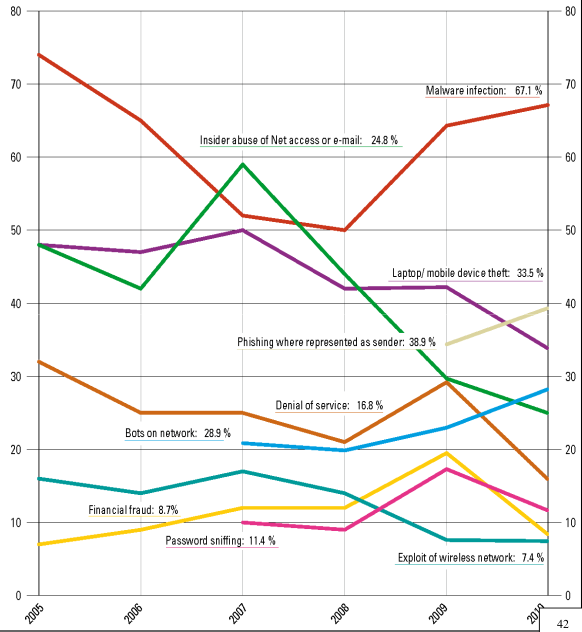
\includegraphics[width = 0.55\textwidth]{chapter1/attacks.png}
  \end{figure}
}{}



\ifthenelse{\boolean{showNew}}{
  \subsection*{Threat model: where is the enemy? Which actions can it perform?}
  \begin{itemize}
    \item \textbf{\emph{MITM} (Main-In-The-Middle):} Sits between two peers A and B;
    \item \textbf{\emph{MATE} (Main-At-The-End):} Resides inside one peer;
    \item \textbf{\emph{MITB} (Main-In-The-Browser):} Resides inside one specific component of one peer (typically the web browser);
    \item \textbf{Passive Attacker:} Can only read the data/traffic;
    \item \textbf{Active Attacker:} Can read, but also modify, delete, or create data/traffic.
  \end{itemize}
}{}

\ifthenelse{\boolean{showOld}}{
  \subsection*{Insecurity: the deep roots}
  \begin{itemize}
    \item "Attack technology is developing in an open-source environment and is evolving rapidly": Most attack tools are released as open-source, making them easily accessible and allowing for rapid development through small improvements.
    \item "Defensive strategies are reactionary": Security measures often lag behind new attack techniques, leaving us vulnerable until new protections are developed.
    \item "Thousands - perhaps millions - of systems with weak security are connected to the Internet": Ensuring the security of all connected computers is essential, as one compromised computer can impact others on the network.
    \item "The explosion in use of the Internet is straining our scarce technical talent. The average level of system administrators has decreased dramatically in the last 5 years.": The increasing use of user-friendly interfaces has led to a decline in technical knowledge, despite improved productivity.Technical expertise is crucial for effective cybersecurity.
    \item "Increasingly complex software is being written by programmers who have received no training in writing secure code": Secure code is critical for preventing vulnerabilities and exploitation. Not all programmers need to be experts in security, but they should be aware of secure coding practices.
    \item "Attacks and attack tools transcend geography and national boundaries.": Investigations often span multiple countries, making it difficult to track down cybercriminals, especially in regions with lax cybersecurity laws.
    \item "The difficulty of criminal investigation of cybercrime coupled with the complexity of international law means that prosecution of computer crime is unlikely.": The complexity of international law and the challenges of investigating cybercrimes often result in a lack of effective prosecution.
  \end{itemize}
}{}


\subsection*{Basic problems (technological)}
\begin{itemize}
  \item The networks are insecure:
        \begin{itemize}
          \item Most communications are made in clear (unless you take some actions);
          \item LANs operate in broadcast (sending messages to everybody, and "if it's not for you, don't read");
          \item Geographical connections are NOT made through end-to-end dedicated lines but through shared lines or through third-party routers.
        \end{itemize}
  \item Weak user authentication (normally password-based);
  \item There is no server authentication;
  \item The software contains many bugs.
\end{itemize}


\section{Some classes of attacks}

\subsection*{Passive and attive attacks}
A useful means of classifying security attacks is in terms of \emph{passive attacks and active attacks}.

A \textbf{passive attack} attempts to {learn or make use of information from the system but does not affect system resources}. Examples of passive attacks are:

\begin{itemize}
  \item \textbf{Packet sniffing:} The content of network packets (e.g., passwords and/or sensitive data) is read by unauthorized parties.
  \item \textbf{Traffic analysis:} Even if the packet content cannot be understood by a third party, an opponent could extract some information about the nature of the communication taking place.
\end{itemize}

An \textbf{active attack} attempts to alter system resources or affect their operation, involving some modification of the data stream or the creation of a false stream. Examples of active attacks are:

\begin{itemize}
  \item \textbf{IP spoofing / shadow server:} Someone uses the address of another host to take its place as a client (and hide its own actions) or as a server.
  \item \textbf{Connection hijacking / data spoofing:} Data is inserted/modified/cancelled during its transmission.
  \item \textbf{Denial-of-service / distributed DoS:} The functionality of a service is limited or disrupted (e.g., ping bombing).
\end{itemize}


\subsection{Packet Sniffing (Eavesdropping)}
\begin{wrapfigure}{r}{0.25\textwidth}
  \centering
  \includegraphics[page = 46,trim = 18cm 2.3cm 0.5cm 11.9cm, clip, width = 0.25\textwidth]{\slides}
\end{wrapfigure}
Packet sniffing refers to reading packets addressed to another network node. It is easy to do in a broadcast network (e.g., LAN) or at switching nodes (e.g., router, switch). This is possible by putting the network card in promiscuous mode, which means that the card will read every packet passing through the device. This kind of attack allows intercepting anything (passwords, data, etc.). Some possible countermeasures are avoid using broadcast networks or encrypt the packet payload (if a non-broadcast network is not possible).


\subsection{Traffic Analysis}
Traffic analysis is more subtle than packet sniffing. Suppose we had a way of masking the contents of messages or other information traffic so that opponents, so that the content of the messages cannot be understood by a third party. Even with encryption in place, the opponent could determine the location and identity of communicating hosts and could observe the frequency and length of messages being exchanged. This information might be useful in guessing the nature of the communication that was taking place.

\subsection{IP Spoofing (Masquerading)}
\begin{wrapfigure}{r}{0.25\textwidth}
  \centering
  \includegraphics[page = 45,trim = 18cm 2.2cm 0.5cm 11.9cm, clip, width = 0.25\textwidth]{\slides}
\end{wrapfigure}
IP spoofing means forging the source network address. Typically, the level 3 (IP) address is forged, but it is equally easy to forge the level 2 address (e.g., ETH, TR, etc.). A better name would be source address spoofing. This is typically used for attacks where an answer is not needed. If everybody is in the same subnet, due to the broadcast function, it is also possible to read the replies. Attacks of this type go for data forging and unauthorized access to systems. The countermeasure for this type of attack is to never rely on address-based authentication: generally, network addresses should not be trusted.

\subsection{Denial-of-Service (DoS)}
Denial-of-service refers to keep a host busy so that it cannot provide its services. For example, in public
administration for a call to a competition, offers can be sent until a date. We can make an offer and stop all the
others from sending email. A possible solution is to send tons of email keeping the server busy until the
message “Message did not deliver because the destination mailbox is full”. We saturated the mail service.
Other examples:
\begin{itemize}
  \item \textbf{Mail/log saturation:} As explained before.
  \item \textbf{Ping flooding ("ping bombing"):} The ICMP echo request usually uses a small number of bits (8 bytes) and starts a timer waiting some seconds for a response. We could use the largest amount of bytes possible: 64 Kbytes. We should send a lot of echo requests at maximum speed without starting timers. This will keep the host busy answering all these packets and prevent it from performing other tasks.
  \item \textbf{SYN flood:} It is a form of denial-of-service attack in which an attacker rapidly initiates a connection to a server without finalizing the connection. The server must spend resources waiting for half-opened connections, which can consume enough resources to make the system unresponsive to legitimate traffic (see TCP SYN flooding).
\end{itemize}

Usually, DoS attacks block the use of a system/device, and there are no countermeasures for it because it is not possible to know if someone connecting to the service is intentionally keeping the service busy or not. In other words, DoS is quite like a high increase in customers using that service. Monitoring and oversizing can mitigate the effects. Every time there is an alert that some threshold is passed, for example, resource saturation, it is time to investigate. It could be a system problem or a security problem. Security and system managers must work together.



\subsection{Distributed Denial-of-Service (DDoS)}

DDoS is essentially the same kind of attack as a DOS attack but magnified by the number of attackers simultaneously targeting a victim.
Typically, a small number of individuals gain control of numerous nodes by installing DoS software on them. Each compromised node is often referred to as a \textbf{daemon, zombie,} or \textbf{malbot}, with the aim of creating a \textbf{botnet}.\\
A botnet is a network of compromised computers (\emph{slaves}) controlled by a \emph{master}. The master typically uses a \textbf{command and control (C\&C)} infrastructure, which can be either client-server or peer-to-peer.
\ul{The communication between the zombies (compromised computers) and the master is often encrypted or routed through "covert" channels}. Covert channels are intended to mislead investigations; for example, information may be concealed by embedding it in \texttt{UDP packets} within \texttt{ICMP Request} messages, making it harder to detect since ICMP messages are common in normal network traffic.

These bots are sophisticated, and there have been cases where they can auto-update themselves to execute new attack techniques; by increasing the number of daemons (compromised computers), the impact of the attack can be magnified.

Other techniques to improve the attack include using a \textbf{"reflector"}. This involves utilizing a potentially legitimate third-party component to relay the attack traffic to the victim. This approach offers two main advantages:
\begin{itemize}
  \item \textbf{It hides the attackers' identities:} attackers send packets to the reflector servers with a source IP address set to their victim's IP (IP spoofing), indirectly overwhelming the victim with response packets.
  \item It \textbf{multiplies the effect} through an \textbf{"amplification factor"} N:1 (typically protocol-dependent),
        where the reflector server's response size is much larger than the request size.
        For example, when making a specific query to DNS, the DNS response can be up to 70 times larger than the request.
\end{itemize}


\subsubsection*{DDOS attack}

\begin{figure}[h]
  \centering
  \includegraphics[page = 49,trim = 0.5cm 2.1cm 1cm 4cm, clip, width = 0.70\textwidth]{\slides}
\end{figure}

There is an attacker and a victim. The attacker somehow creates a network of daemons, then selects some nodes to be masters (usually more than one for redundancy), which are part of the botnet. The attacker sends the IP address to attack and then \emph{disconnects from the network} to avoid being tracked. The other masters will coordinate the work of the daemons, which must perform the attack at the same time. Masters do not directly take part in the attack; they try to remain hidden as much as possible to avoid being detected during an investigation because this would stop the attack. The huge class of amplification factors that daemons can create can overwhelm the victim.

Masters and daemons are not real individuals but part of the botnet. The only human involved is the attacker, who disconnects after initiating the DDOS attack.


\subsubsection*{Case History: DDoS towards Yahoo Server Farm}

The first well-known attack of this kind occurred on Feb 8th, 2000, at 10:30 am (PST) against the Yahoo Server Farm. Administrators wrote a report that stated:
\begin{itemize}
  \item "The initial flood of packets, which we later realized was in excess of 1 Gbit/sec, took down one of our routers..."
  \item "... after the router recovered, we lost all routing to our upstream ISP..." This happened because an internet connection requires two routers. Yahoo's people rebooted their own router, but at the other end of the communication link, the router was still down.
  \item "... it was somewhat difficult to tell what was going on, but at the very least, we noticed lots of ICMP traffic..."
  \item "... at 1:30 pm, we got basic routing back up and then realized that we were under a DDoS attack."
\end{itemize}
Later, the attack was traced back to the 15-year-old Canadian boy Michael Calce (aka MafiaBoy). Even if getting to the attacker is not always possible, a U.S. lawyer can easily identify who the daemons are and seek refunds from them, even if the daemon was a victim of the attacker, for example, if the attacker took control of a computer for DDoS purposes.



\ifthenelse{\boolean{showOld}}{
  An interesting legal implication for zombie nodes: "Be Secure or Be Sued":
  \begin{quote}
    "There is a distinct probability that if your site has been hijacked for a denial of service attack, then you could be liable for damages. I would definitely advise clients they have grounds to sue."
    \begin{flushright}
      Nick Lockett, an e-commerce lawyer at Sidley \& Austin.
    \end{flushright}
  \end{quote}
}{}

\subsubsection*{Case History: DDoS towards "Krebs on Security" Blog}
On September 27, 2016, the administrator of the blog received a DDoS attack that generated 665 Gbps, and it was generated by a botnet of IoT devices (or claimed to be such).
There was no use of any reflectors or amplifiers, just millions of devices that performed perfectly valid requests.
It seemed like millions of users wanted to connect to the website at the same time. This generated a significant amount of traffic, and even though the blog was hosted on Akamai, the traffic was so substantial that the company had to give up and made the blog unreachable by dropping that destination from their routing table on September 29.
There was no known reason for the attack; perhaps it is connected to Krebs' analysis of similar attacks against online game servers.


\subsection{Shadow Server / Fake Server}
In \textbf{shadow server} attacks, a host manages to impersonate itself as a service provider to victims without having the right to do so. There are two techniques to achieve this:
\begin{itemize}
  \item If the attacker \textbf{can sniff requests and spoof responses faster than the real server}, the latter will not be able to communicate because the second package will be discarded, considering it a duplicate.
  \item \textbf{Routing or DNS manipulation}, mapping the real name to the IP of the shadow server.
\end{itemize}

The attacks that can be carried out in these scenarios include:
\begin{itemize}
  \item \textbf{Issuing incorrect answers}, providing a "wrong" service to victims instead of the real one.
  \item \textbf{Capturing victim's data} provided to the wrong service.
\end{itemize}
The countermeasure to this type of attack is to \textbf{require server authentication}.


\subsection{Connection Hijacking / Man In The Middle (MITM)}
It is also referred to as \textbf{data spoofing}, and this form of attack involves gaining control of a communication channel to insert, delete, or manipulate the traffic. This can be achieved through logical means (by altering the network's routing) or physically (if one can physically access a router or switch).

These attacks can be executed for various reasons, such as eavesdropping, inserting false data, and altering data exchanged between two parties.


Countermeasures include \textbf{authentication}, ensuring data \textbf{integrity} (verifying whether it has been altered), and packet \textbf{serialization} (ensuring that no packets are added or deleted, and that packets are received in the same manner as they were sent) \ul{for each individual network packet}.



% TODO: from here, virus and others are added as section.
% section or subsection?

\subsection{Trojan}
A Trojan is a program that hides a malicious payload within a seemingly harmless exterior. Despite the increasing security of network channels, user terminals have become more susceptible to such attacks. This vulnerability extends to devices like smartphones, smart TVs, and various Internet of Things (IoT) devices.

These attacks tend to target less tech-savvy or "ignorant" users. Attack tools can take on various forms, from traditional methods like embedding keyloggers within seemingly innocuous applications to more contemporary approaches, such as malicious browser extensions.

Trojans are frequently used to carry out two distinctive types of attacks: \textbf{"Man-At-The-End"}(\emph{MATE}) and \textbf{"Man-In-The-Browser"} (\emph{MITB}).


\subsection{Zeus}
The Zeus attack, also known as \textbf{Zbot}, is a major malware threat combined with a botnet. It was first discovered in 2007, and law enforcement has been actively seeking the owner of this network. The owner claimed to have sold it in 2010.

Zeus can be used in the following ways:
\begin{itemize}
  \item Directly: For example, it can be employed for Man-In-The-Browser (MITB) attacks to perform keylogging or form grabbing (software that reads data in a form).
  \item Indirectly: It can also be used to deliver other malware, such as the CryptoLocker ransomware.
\end{itemize}

Zeus is challenging to detect and remove because it employs stealth techniques to conceal itself. In the USA alone, there are approximately 3.6 million active copies of Zeus.


\subsection{Software Bug}
Even the best software can have bugs, which can be exploited for various purposes. One common way to exploit a software bug is to create a Denial of Service (DoS) attack.

For instance, there was an attack against the WinNT server (versions 3.51 and 4.0) where attackers discovered that the server hosted a service on an undocumented TCP port 135. They attempted to communicate with this port by sending 10 random characters followed by a carriage return (CR). This caused the server to become unavailable, as it experienced 100\% CPU load even though it was not performing any useful work.

The issue stemmed from the fact that at port 135, there was a new Microsoft-only service that was a remote procedure call (RPC) and had a bug. When it received a malformed packet, it went into an infinite loop, continuously asking, "where is a good packet?" Since the ARP server (?) was part of the operating system's kernel, it consumed 100\% of the CPU without the possibility of interruption. Microsoft developed a solution with Service Pack 3 (SP3), in which they addressed and corrected this bug.


\ifthenelse{\boolean{showOld}}{
  \subsection*{Some Typical Application-Level Problems}
  \begin{itemize}
    \item \textbf{Buffer Overflow}:
          \begin{itemize}
            \item Occurs when a programmer allocates a memory buffer without verifying that the data being stored does not overflow that allocated memory. This can allow an attacker to inject malicious code.
          \end{itemize}
    \item \textbf{Storing Sensitive Information in Cookies}:
          \begin{itemize}
            \item This can expose sensitive information to third parties, either during transit or locally on the client.
          \end{itemize}
    \item \textbf{Storing Passwords in Clear Text in a Database}:
          \begin{itemize}
            \item This practice makes passwords readable by third parties, such as backup operators responsible for data copies.
          \end{itemize}
    \item \textbf{"Invent" a protection system}:
          \begin{itemize}
            \item The issue here lies in the potential risks associated with inadequate protection.
          \end{itemize}
  \end{itemize}
}{}


\section{Virus \& Co. (malware)}
\begin{itemize}
  \item \textbf{Virus}:
        A virus is a malicious program that damages the target and then duplicates itself. It is propagated by humans involuntarily.
  \item \textbf{Worm}:
        A worm damages the target indirectly by replicating itself to the extent that it achieves resource saturation. Additionally, a worm will attempt to propagate automatically. Worms are usually more challenging to detect because the damage they cause may resemble normal activity unless a careful analysis of the network pattern is conducted.
  \item \textbf{Trojan Horse}:
        The Trojan horse is a program that carries some malware. It may appear to be a valid program but can also install malware.
  \item \textbf{Backdoor}:
        A backdoor is a piece of software that provides an unauthorized access point. While illegal, it is common among developers. For example, if a developer is concerned about not being paid, they might create a backdoor to gain access in case of payment problems.
  \item \textbf{Rootkit}:
        A rootkit is a set of tools that provides privileged access. It is hidden, often disguised as a modified program, library, driver, kernel module, or hypervisor. Due to its stealthy nature, rootkits are challenging to detect and remove.
  \item \textbf{PUA (Potentially Unwanted Applications)}:
        It's a sort of grayware, not directly dangerous.
\end{itemize}


\subsection*{Virus and worm (malware)}
Virus and worms require some kind of complicity (may be involuntary) from \textbf{the user} (gratis, free, urgent,
important), the \textbf{system manager} (wrong configuration), \textbf{the producer} (automatic execution, trusted).

Some countermeasures are user awareness, correct configuration/secure software, antivirus (installed and updated).


\subsection*{Malware food chain}
\begin{wrapfigure}{r}{0.40\textwidth}
  \centering
  \includegraphics[page = 60,trim = 1cm 2cm 1cm 5cm, clip, width = 0.40\textwidth]{\slides}
\end{wrapfigure}
When someone discovers a vulnerability, it can be exploited for the development of malicious code (for example, this code could be used to gain access to a website and manipulate its data). Such information can be exploited in two ways:
\begin{itemize}
  \item Especially in the past some individuals may perform the attack primarily for the sake of recognition, like being in a "Hall of Fame".

  \item More recently, individuals have been motivated by business interests. They sell the information about the vulnerability or a working code that exploits it on the \emph{vulnerability marketplace}, a hidden marketplace and is found exclusively on the internet, on dummy servers that appear for a brief time during the night.
\end{itemize}

Payment for these vulnerabilities is often made using cryptocurrency. The buyers of these vulnerabilities are typically the \textbf{malware toolkit makers}, which are used to develop attack programs that incorporate malware; malware distributors, such as spammers and website owners, then employ this type of software for their illicit activities.


\subsubsection*{Zeus: Cyber Theft Ring}
"It often happens to receive an email that asks you to send money outside of the country in exchange for a large sum of money. If you accept this request, you will supposedly receive the money. They may begin by testing you, sending a small amount of money, for example, \$10,000, and then ask you to send \$7,000 to Nigeria, allowing you to keep \$3,000 for yourself. However, by agreeing to this, you will be facilitating money laundering, as the funds are stolen from someone's bank account and transferred to you, making you appear responsible. You will then send the money via MoneyGram, while the individuals in Nigeria will disappear, leaving you to face potential legal consequences. This scenario is a typical case of acting as a 'money mule,' which involves accepting funds from a stolen bank account and forwarding them to the intended destination."